\chapter[Proposta]{Proposta}
O objetivo deste capítulo é apresentar uma possível proposta de uma solução que atenda às necessidades colocadas no primeiro capítulo referente a problemática deste trabalho. A proposta está dividida em duas partes. A primeira parte está relacionada à coleta das métricas utilizando a ferramenta SonarQube, e a segunda parte está relacionada na criação do \textit{dashboard} e a visualização das informações. Para analise deste projeto foram escolhidos dois projetos, sendo o projeto PROJETO 1 e o PROJETO 2 de código aberto DO ORGAO como base para elaboração deste trabalho. A terceira e última parte do tarabalho consiste em analisar o trabalho realizado através de uma avaliação qualitativa de possíveis usuários.
\section{Coleta das Métricas}
Para fazer a coleta das métricas vai ser utilizado a ferramenta SonarQube que como já dito na seção de Suporte Tecnológico é muito utilizado em órgãos públicos e em editais por ser uma ferramenta \textit{open-source}. A coleta das métricas é feita com base no edital feito pelo DNPM \cite{edital} que se baseia na Suíte de Métricas de Chidamber-Kemerer. As métricas e suas metas estão apresentadas a seguir.
\begin{itemize}
\item Taxa de Cobertura de Teste Unitário = 80;
\item LCOM 4 = 10;
\item Violações do tipo Blocker = 0;
\item Violações do tipo Critical = 0;
\item Violações do Tipo Major = 0,5 total de linhas de código;
\item Violações do Tipo Minor = 1 total de linhas de código;
\item Taxa de Duplicações de blocos = igual ou menor que 2 total de linhas de código;
\item Linhas de Código Comentadas = igual ou menor que 1 do total de linhas de código;
\item WMC;
\item DIT;
\item NOC;
\item RFC;
\item CBO.
\end{itemize}
O objetivo deste trabalho é criar uma ferramenta que auxilie na auditoria de software entregue por empresas tercerizadas, contudo é percebe-se que ainda que o trabalho possua grande aprovação ele nunca substituira o fator humano da auditoria, o software serve apenas como uma ferramenta de avaliação geral do software entregue. Recomenda-se que uma vez que o software seja submetido à ferramenta e seja aceito é necessário que seja feita uma auditoria em cima de uma amostragem do software entregue sob o olhar de um analista especializado para tal atividade.
\\Uma vez analisado o projeto utilizando o Sonar Scanner um relatório é grerado e este relatório é exportado em formato XML para ser utilizado pela ferramenta desenvolvida neste trabalho. Uma segunda alternativa para capturar as informações geradas pelo Sonar seria utilizar o plugin Report do SonarQube para capturar a informação. Uma terceira alternativa seria criar um script python que leia a pagina html do sonarqube e através de expressão regular separar as informações da página.
\\As métricas "Violações do tipo Blocker", "Violações do tipo Major" e "Violações do tipo Minor" são estipuladas de acordo com o próprio perfil do Sonar, chamado Sonar Way. Contudo a melhor maneira seria criar um perfil com as regras da própria organização garantindo uma avaliação mais focada no objetivo do orgão.
\section{Criação do \textit{Dashboard}}
Com as informações obtidas o dashboard funcionará como uma tela para visualização dessas métricas. A solução é composta por duas telas, uma mostrando uma visão geral do projetos, e com indicadores quanto aprovação ou reprovação de cada projeto seguindo os limites estabelecidos pelo edital \cite{edital} que é de onde está sendo baseado as métricas e limites dos indicadores. A segunda tela consiste em uma visão mais detalhada sobre cada projeto mostrando a evolução do projeto em cada métrica e com um \textit{link} para o Sonar de cada métrica para um aprofundamento.

\section{Avaliação}
A avaliação do \textit{dashboard} será feita por parte de um gestor de tecnologia de um orgão público. Ele avaliará aspectos de usabilidade da ferramenta e se a ferramenta possuiria condições mínimas de ser implantada. Caso não seja possível essa avaliação com um profissional da área a avaliação será feita através de professores que possuem tal experiência com contratação de software para orgãos públicos também avaliando aspectos como usabilidade e melhorias necessárias para implantação em um orgão.
Para fazer está avaliação o gestor responderá a um questionário contendo 15 perguntas referentes ao uso e funcionalidades do software produzido. O questionário é igual ao da imagem \ref{img:questionario}

\graphicspath{{figuras/}}
\begin{figure}[h]
\centering
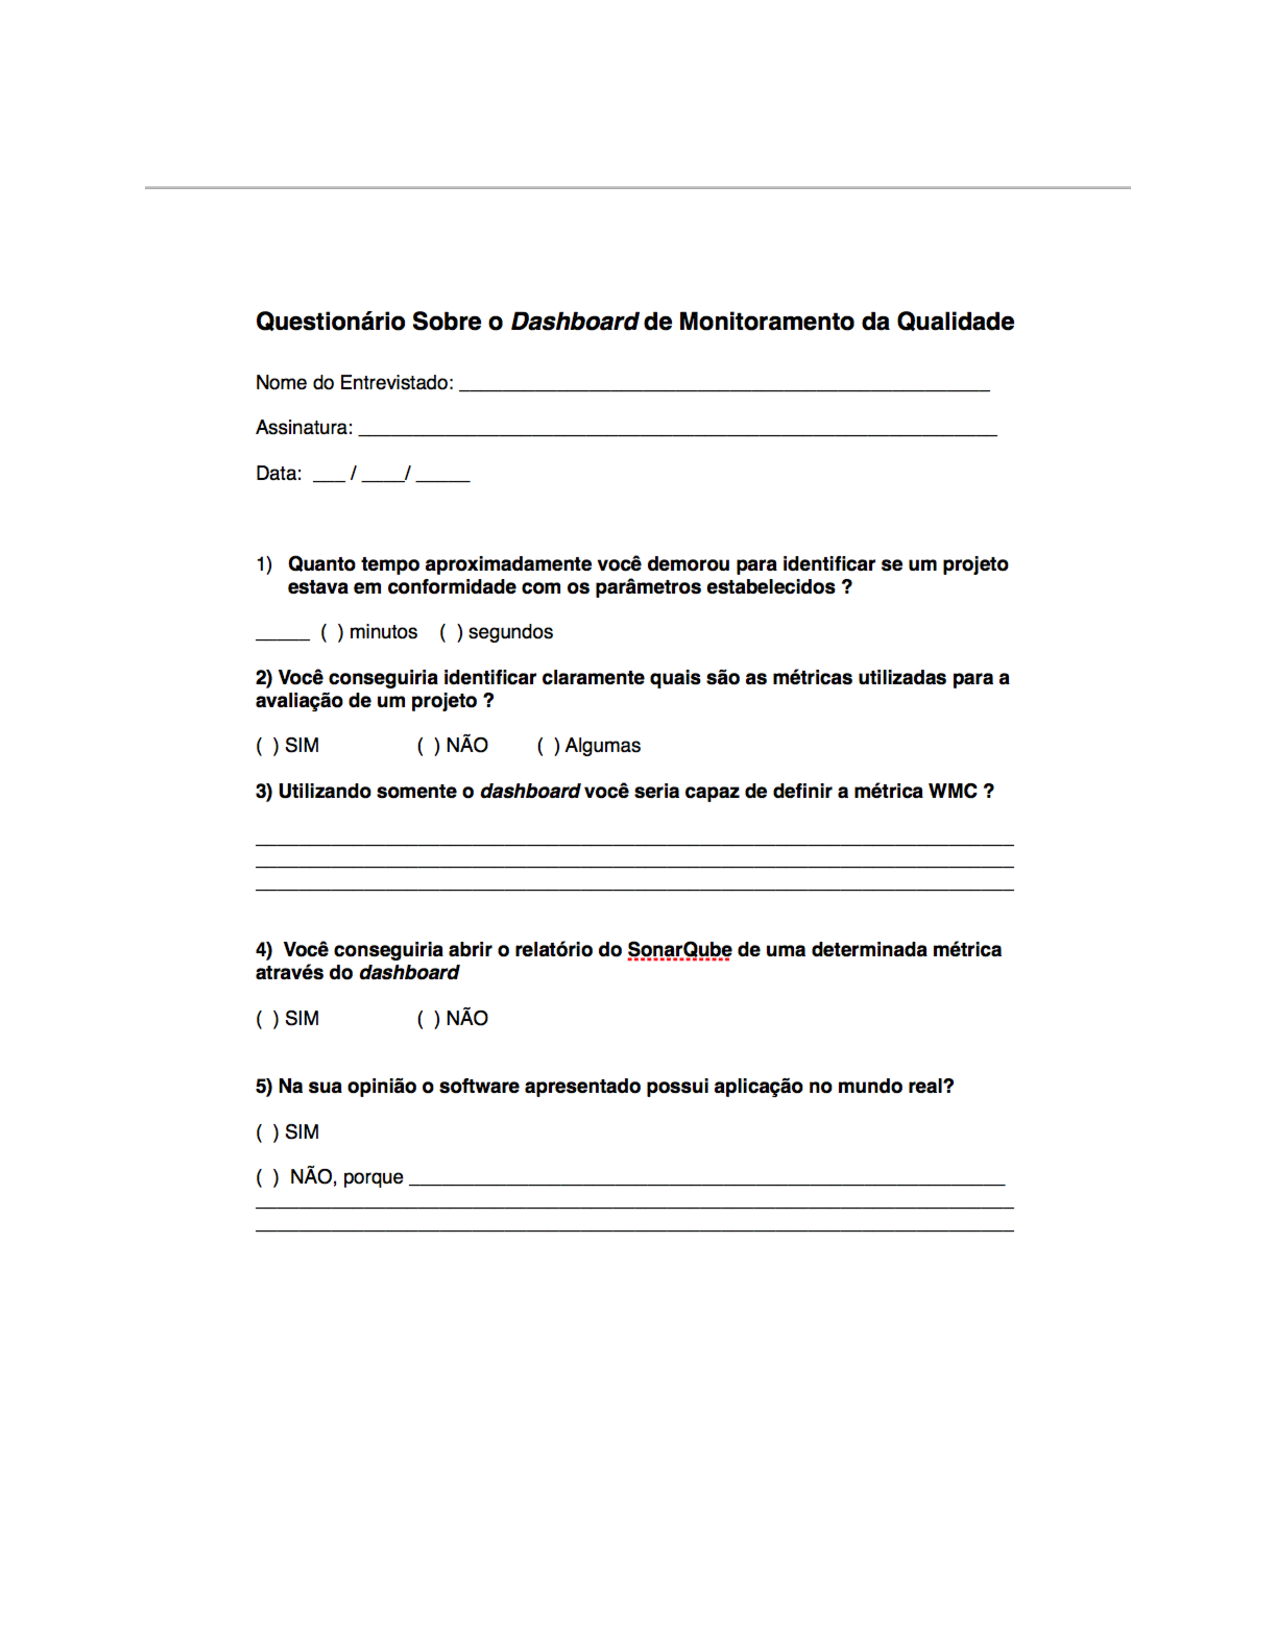
\includegraphics[scale=1.00]{questionario}
\caption{Questionário a ser aplicado ao fim do período de teste}
\label{img:questionario}
\end{figure}

\section{Resumo do Capítulo}
Inicialmente será criada uma instancia da ferramenta SonarQube que coletará as métricas nos projetos indicados. Quando essas métricas tiverem sido coletadas será gerado um arquivo XML contendo o nome do projeto, a métrica e o valor coletado. Esta primeira etapa é dada concluida quando XML for gerado. Para a segunda etapa é criado um \textit{dashboard} onde será possível acompanhar dois projetos de software. O objetivo desta etapa é ter uma visão se um determinado projeto está dentro dos padrões estipulados ou não, para isto os projetos serão sinalizados quando estiverem em falta com alguma métrica. A última etapa deste trabalho consiste na avaliação do trabalho produzido que será feito juntamente com um gestor de projeto de um órgão público que responderá a um questionário quanto ao software.